% !TeX root = 00_cep_semantics.tex
\appendix
\section*{Appendix A. Category-Theoretic Background}
\addcontentsline{toc}{section}{Appendix A. Category-Theoretic Background}

This appendix summarizes the categorical notions used in the paper.
It is intended for readers familiar with structured data, provenance, or
formal methods who may not work with category theory daily.
The goal is conceptual clarity rather than mathematical depth.

% ------------------------------------------------------------
\subsection*{A.1 Categories}
% ------------------------------------------------------------

A \emph{category} consists of:
\begin{itemize}
  \item a collection of \textbf{objects};
  \item a collection of \textbf{morphisms} (arrows) between objects;
  \item identity morphisms and an associative composition operation.
\end{itemize}

Intuition:
\begin{itemize}
  \item Objects represent structured states (e.g., CEP records).
  \item Morphisms represent valid transformations (e.g., amendments).
  \item Composition corresponds to performing transformations in sequence.
\end{itemize}

Example: a sequence of CEP record updates is a chain of morphisms
\[ R_0 \to R_1 \to R_2 \to \cdots. \]

% ------------------------------------------------------------
\subsection*{A.2 Functors}
% ------------------------------------------------------------

A \emph{functor} $F : \mathbf{C} \to \mathbf{D}$ maps:
\begin{itemize}
  \item each object of $\mathbf{C}$ to an object of $\mathbf{D}$;
  \item each morphism of $\mathbf{C}$ to a morphism of $\mathbf{D}$;
\end{itemize}
while preserving identities and composition.

Intuition:
\begin{itemize}
  \item A functor expresses a structure-preserving translation.
  \item CEP uses functors to model envelope construction,
        canonicalization, and provenance propagation.
\end{itemize}

% ------------------------------------------------------------
\subsection*{A.3 Natural Transformations}
% ------------------------------------------------------------

Given functors $F, G : \mathbf{C} \to \mathbf{D}$,
a \emph{natural transformation} $\eta : F \Rightarrow G$
assigns to each object $X$ a morphism
\[
  \eta_X : F(X) \to G(X)
\]
such that for every $f : X \to Y$ the square
\[
  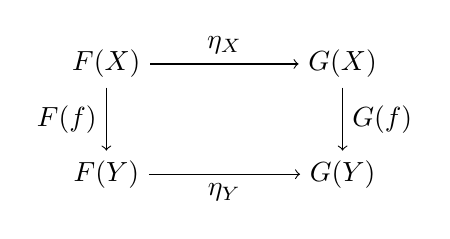
\begin{tikzpicture}[baseline=(current bounding box.center)]
    \node (FX) at (0,0) {$F(X)$};
    \node (GX) at (3,0) {$G(X)$};
    \node (FY) at (0,-1.4) {$F(Y)$};
    \node (GY) at (3,-1.4) {$G(Y)$};
    \draw[->] (FX) -- node[above] {$\eta_X$} (GX);
    \draw[->] (FY) -- node[below] {$\eta_Y$} (GY);
    \draw[->] (FX) -- node[left] {$F(f)$} (FY);
    \draw[->] (GX) -- node[right] {$G(f)$} (GY);
  \end{tikzpicture}
\]
commutes.

Intuition:
\begin{itemize}
  \item Naturality expresses the compatibility condition:
        \emph{``attest then update'' = ``update then attest''}.
  \item This coherence underlies CEP envelope and attestation chains.
\end{itemize}

\medskip
The categorical tools summarized in this appendix correspond directly to
the rewriting-based normalization pipeline developed in the main text.
Categories and functors model record states and their admissible
transformations; monoidal structure captures the ordered concatenation of
canonical components; oplax functors express structure-weakening
translations such as jurisdictional adapters; and fibrations formalize
how context tags vary over identity-bearing records.
The stratified ordering of rewrite rules in canonicalization aligns with these
structures: each stratum corresponds to a functorial transformation, and
the monoidal product enforces the fixed sequencing required for
deterministic normalization.
\medskip


% ------------------------------------------------------------
\subsection*{A.4 Monoidal Categories and Stratified Rewriting}
% ------------------------------------------------------------

A \emph{monoidal category} is a category equipped with:
\begin{itemize}
  \item a tensor product $\otimes$,
  \item a unit object $I$,
  \item coherence laws for associativity and unit behavior.
\end{itemize}

In CEP, the monoidal structure is string concatenation:
\begin{itemize}
  \item canonical components (name, address, date, jurisdiction)
        combine via $\otimes$;
  \item the canonicalization functor preserves this structure strictly.
\end{itemize}

This yields determinism in canonical string construction and hence in SNFEI identifiers.

In CEP, the monoidal product reflects the ordered application of rewrite
strata in the normalization pipeline, ensuring that semantic expansions,
structural simplifications, and surface-level normalizations compose deterministically.

% ------------------------------------------------------------
\subsection*{A.5 Oplax Functors}
% ------------------------------------------------------------

Given monoidal categories $(\mathbf{C}, \otimes)$ and $(\mathbf{D}, \otimes)$,
an \emph{oplax monoidal functor} $F : \mathbf{C} \to \mathbf{D}$ includes
coherence maps
\[
  F(X) \otimes F(Y) \to F(X \otimes Y)
\]
that are not required to be isomorphisms.

Intuition:
\begin{itemize}
  \item Oplax functors allow \textbf{structure weakening}.
  \item This models jurisdictional adapters: local structure may map
        incompletely or partially into the global vocabulary.
\end{itemize}

% ------------------------------------------------------------
\subsection*{A.6 Indexed Families and Fibrations}
% ------------------------------------------------------------

A \emph{fibration} $\pi : \mathbf{E} \to \mathbf{B}$ consists of:
\begin{itemize}
  \item a base category $\mathbf{B}$,
  \item a total category $\mathbf{E}$,
  \item a projection functor $\pi$,
  \item satisfying certain lifting properties.
\end{itemize}

The fiber over $B \in \mathbf{B}$ is the category
\[
  \mathbf{E}_B = \{ E \in \mathbf{E} \mid \pi(E) = B \}.
\]

Intuition for CEP:
\begin{itemize}
  \item $\mathbf{B} = \mathbf{CEP}$ (identity-bearing records),
  \item $\mathbf{E} = \mathbf{CT}$ (records with context tags),
  \item the fiber over $R$ contains all valid tags for $R$,
  \item reindexing tracks tag evolution without altering identity.
\end{itemize}

% ------------------------------------------------------------
\subsection*{A.7 Universal Properties (Informal)}
% ------------------------------------------------------------

A universal property characterizes an object uniquely (up to isomorphism)
by its relationships to other objects.

In CEP:
\begin{itemize}
  \item the canonical string is universal for its class of normalized components,
  \item the SNFEI arises from applying a hashing endofunctor,
  \item identity preservation follows from the uniqueness of this construction.
\end{itemize}

\bigskip
Further reading: Mac~Lane~\cite{maclane1971categories},
Awodey~\cite{awodey2010category},
Spivak~\cite{spivak2014category}.
